% Created 2024-02-07 Mi 23:50
% Intended LaTeX compiler: pdflatex
\documentclass[a4paper]{article}
\usepackage[utf8]{inputenc}
\usepackage[T1]{fontenc}
\usepackage{graphicx}
\usepackage{grffile}
\usepackage{longtable}
\usepackage{wrapfig}
\usepackage{rotating}
\usepackage[normalem]{ulem}
\usepackage{amsmath}
\usepackage{textcomp}
\usepackage{amssymb}
\usepackage{capt-of}
\usepackage{hyperref}
\author{Dr.-Ing. Amir Najafi, Abdul Aziz}
\date{\today}
\title{Power Planning and IR Drop Analysis}
\hypersetup{
 pdfauthor={Dr.-Ing. Amir Najafi, Abdul Aziz},
 pdftitle={Power Planning and IR Drop Analysis},
 pdfkeywords={},
 pdfsubject={},
 pdfcreator={Abdul Aziz_Project SoSe23}, 
 pdflang={English}}
\begin{document}

\maketitle
\tableofcontents

\noindent\rule{\textwidth}{0.5pt}
\section{Goal}
\label{sec:orgd60c190}
This document contains information on power planning and IR drop analysis. Specifically, it cointains:
\begin{itemize}
\item Theory and math related to power and rail analysis.
\item Practical know-how on doing rail and power analysis using EDA tools.
\item New technologies for IR drop reduction.
\item State of the art approaches for IR drop estimation using AI.
\end{itemize}

\section{Theory}
\label{sec:org80b567a}
\url{https://www.ansys.com/blog/minimizing-ir-drop-in-integrated-circuit-design}

\url{https://www.vlsi-expert.com/2017/12/vias.html}

\begin{itemize}
\item liberty file explanation(.lib) or timing files
\end{itemize}
\url{https://www.vlsisystemdesign.com/worried-about-liberty-basics-lets-start-from-ground-zero/}

\begin{itemize}
\item STA
\end{itemize}
\url{https://github.com/brabect1/sta\_basics\_course/blob/master/doc/sta\_basics\_course.rst\#static-timing-analysis}

\begin{itemize}
\item File
\end{itemize}
\url{https://eternallearning.github.io/phys-synthesis-and-optimization/}


\begin{itemize}
\item Path delay
\end{itemize}
It is refer to the time, it takes for a signal to travel from one point to another point (destination).

\begin{itemize}
\item Mapping
\end{itemize}
The goal of mapping is to transform a technology-independent description of a logic circuit into a technology specific reprentation


\subsection{What is IR Drop?}
\label{sec:org78c9896}

The potential difference,or voltage drop, between two ends of a conducting
wire during current flow is called IR drop (from Ohm’s law: V=IR).
In chips, power and ground are distributed through metal networks
constituting the power delivery networks (PDNs). When current flows
through the PDN, part of the voltage is dropped across the network,
as per Ohm’s law. This phenomenon is called IR drop.

This voltage drop in the power delivery network before
the voltage reaches standard cell
power pins significantly affects the chip's switching speed and performance.
The same effect on the ground net leads to ground bounce, in which
the nominally zero voltage rises above zero.


\subsection{Why IR drop analysis is important?}
\label{sec:orgca941d0}
\begin{itemize}
\item Excessive IR drops degrades the circuit performence.
\item Leads to functional failure
\item Some ATPG test vectors causes excessive IR drop that results yield loss.
\end{itemize}


\subsection{Types of IR drop analysis}
\label{sec:org9bc8d41}
\begin{itemize}
\item Static IR drop
\begin{itemize}
\item Based on leackage power of transistor or standard cell.
\end{itemize}
\item dynamic IR drop
\begin{itemize}
\item vectorless
\item vectorbased
\end{itemize}
\end{itemize}

\noindent\rule{\textwidth}{0.5pt}

\section{Literature Review}
\label{sec:orgcd3e47e}
A summary of books, papers, or online articles;

\subsection{paper 1: IncPIRD. Fast learning-based prediction of Incremental IR drop.}
\label{sec:orgf776efd}
\begin{itemize}
\item denser power grid. for ir requirements and spaser power grid. to give more routing resources
\item by using superposition and partitioning techniques, it is possible to extract electrical features- given soc floorplan and PDN.
\item using a mchine learning model to predict the updated static IR drop for each power node -having tap current source attached
\item Traditional way of ir violation fixing:
\item macro/cell block movement
\item macro/cell block change
\item modification of PDN to have a denser grid
\item adding/moving power pads
\item reduce overdesigned PDN resources by replacing with sparser PDN grids
\item removing power pads

\item input/given: LEF, DEF current distribution, technology file, IR drop file, power pad file of floorplan after modifications.
\end{itemize}


\subsection{paper 2: ML based Dyn IR drop pridiction for ECO*}
\label{sec:orgb93b7e8}

\begin{itemize}
\item Why ECO:
\item 1.Dsign corrections and modifications
\item 2.Cost and time efficiency
\item 3.iterative design process
\item 4.Changing requirements
\item 5.Compatibility issues
\item 6.Regulatory Compliance
\item 7.Bug Fixes
\item 8.Optimizations
\item Eco plays a crucial role on physical design.This helps manage costs, save time and adapt to evolving project requirements.
\end{itemize}

In the time of ECO design sign off, many iteration needed
this means long time required.
Waste of reresources.
Repeated dynamic IR drop simulations.

\begin{figure}[htbp]
\centering
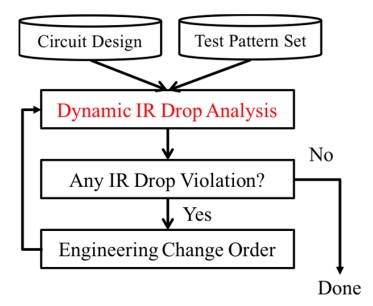
\includegraphics[width=.9\linewidth]{./img/p0.jpg}
\caption{\label{fig:org3af54b6}Traditional IR Drop signoff flow}
\end{figure}

\begin{figure}[htbp]
\centering
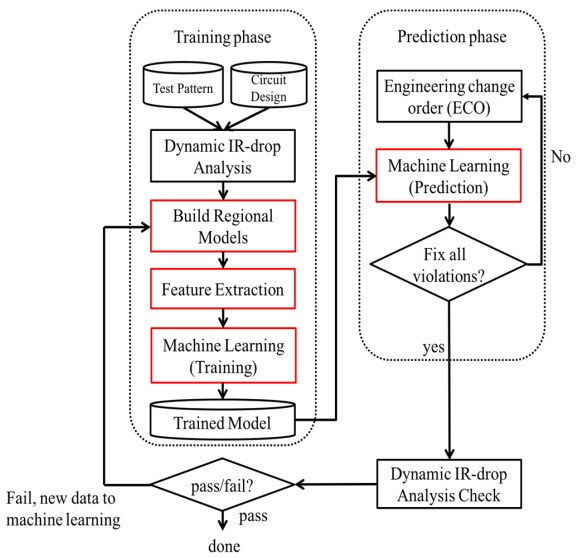
\includegraphics[width=.9\linewidth]{./img/p2.jpg}
\caption{\label{fig:org47c2be0}Model training(left) and prediction flow}
\end{figure}


\begin{figure}[htbp]
\centering
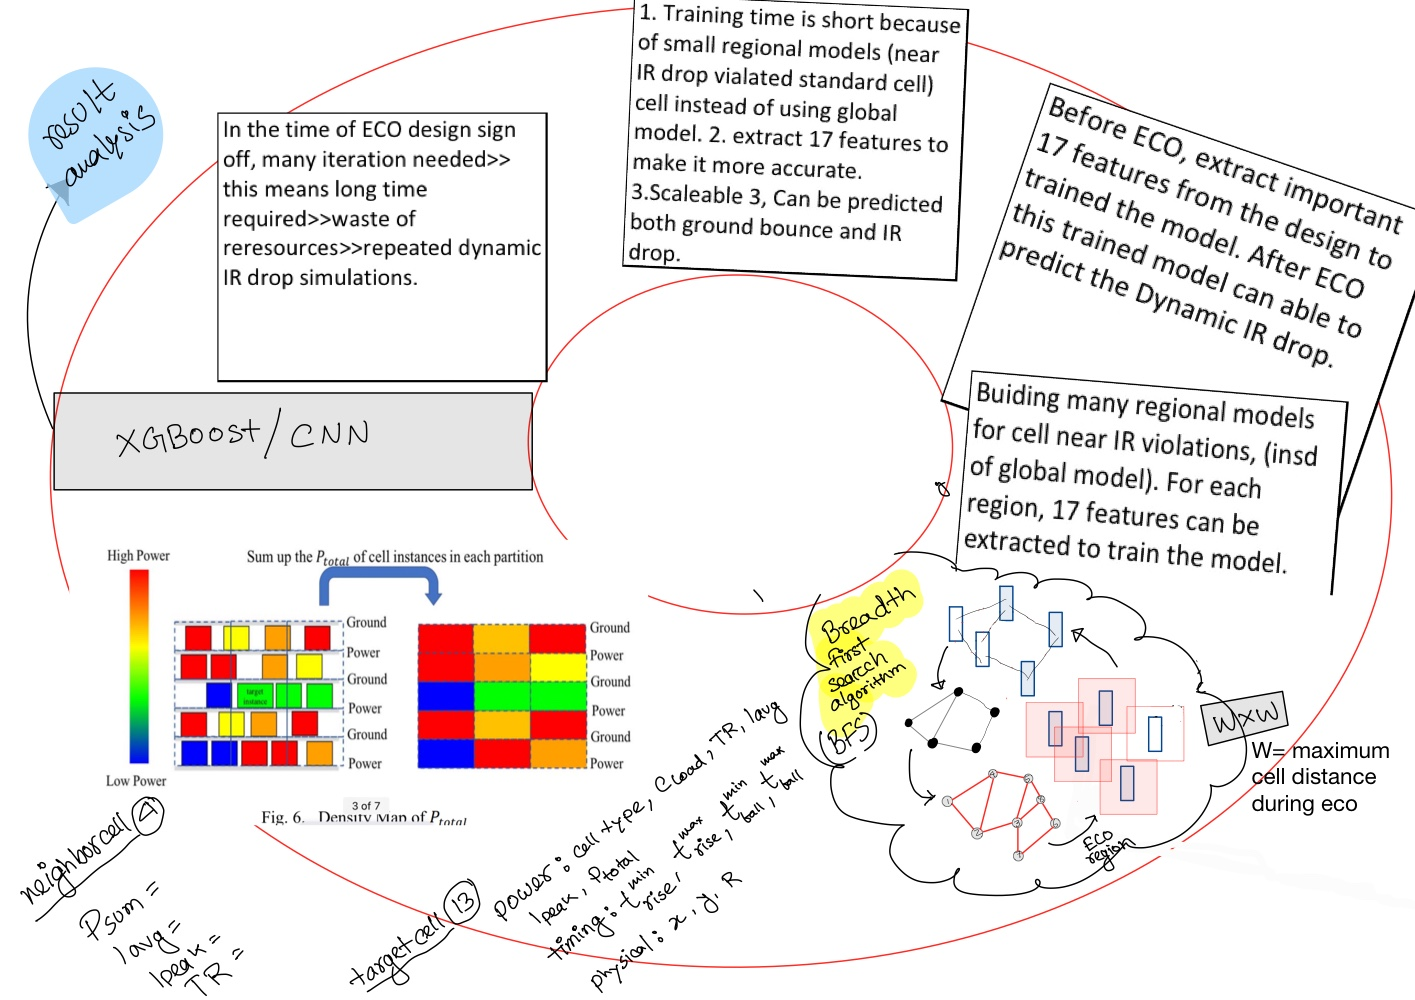
\includegraphics[width=.9\linewidth]{./img/p4.JPG}
\caption{\label{fig:org91e31c4}Model training(left) and prediction flow}
\end{figure}


\begin{figure}[htbp]
\centering
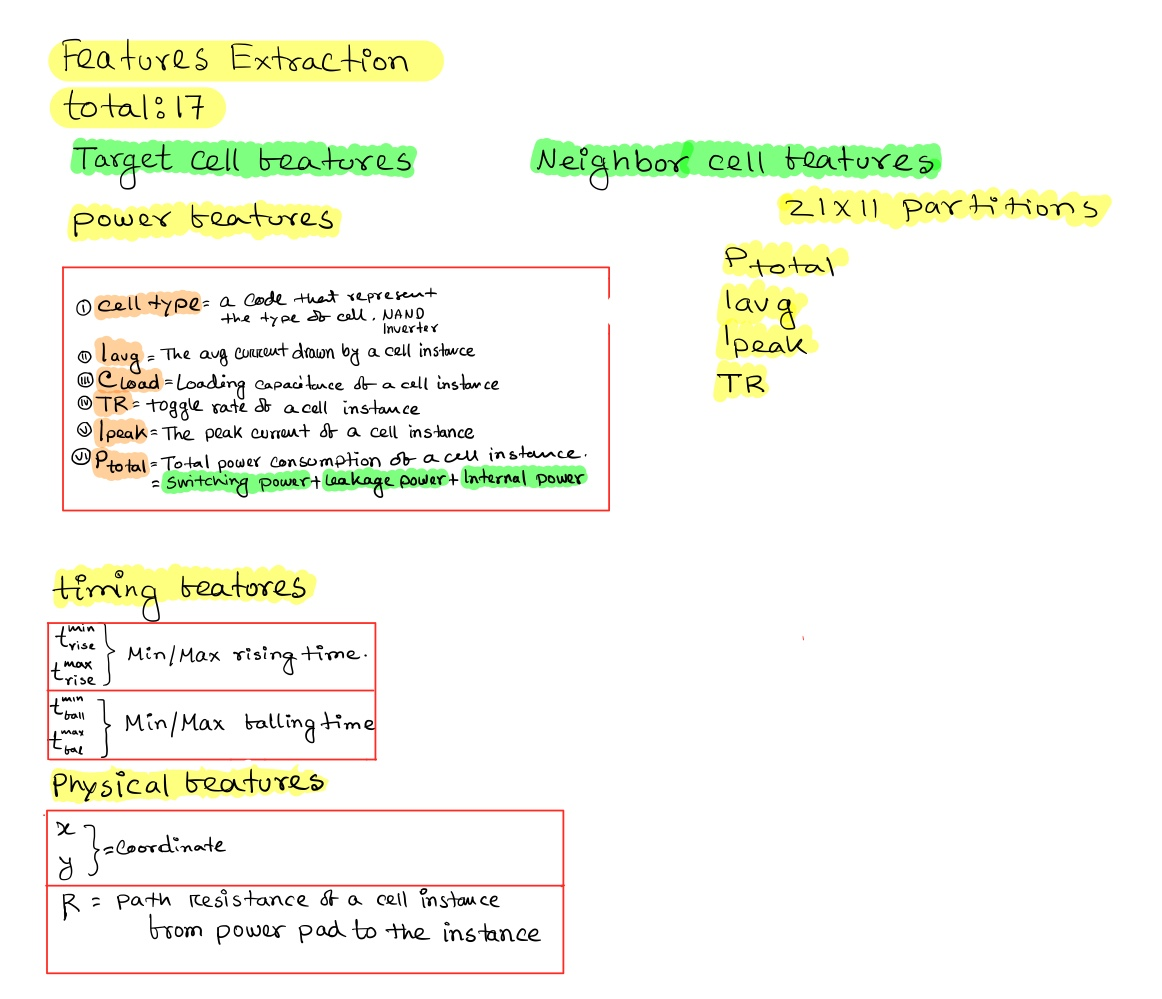
\includegraphics[width=.9\linewidth]{./img/p3.JPG}
\caption{\label{fig:orgf94de3a}Features extraction}
\end{figure}



\begin{itemize}
\item W= maximum distance that a cell instance may move during ECO.
\item cell instance/power node should be stayed in the small region
every IR drop violation will be calculated in (WXW)
\end{itemize}

\begin{figure}[htbp]
\centering
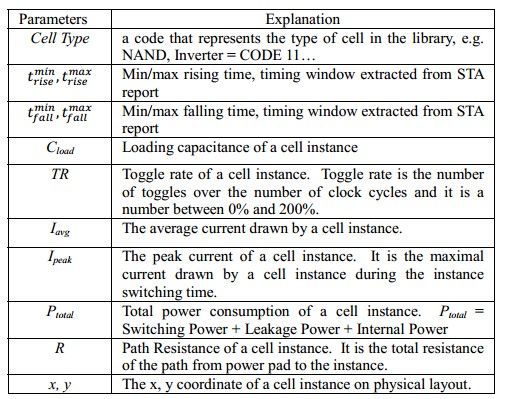
\includegraphics[width=.9\linewidth]{./img/p1.jpg}
\caption{\label{fig:orgfa4f187}This is the caption for the next figure link (or table)}
\end{figure}


\subsection{paper 3: Vector-based Dynamic IR-drop prediction Using ML}
\label{sec:org405f5f9}

\begin{itemize}
\item Motivation:
Long simulation time of vectorbased dynamic IR drop analysis
No such good methods to identify IR-drop risky vectors
\item Goals:
Predict vector-based* dynamic IR drop for all cells
Identify IR-drop risky vectors quickly

\item Inputs:

\item Outputs:

\item Technical terms
IR drop risky vector:

\item MIMO Chart
\end{itemize}

\begin{center}
\begin{tabular}{lll}
Input &  & + output\\
GDSII &  & + vectorprofile.rpt\\
tech lib .cl &  & + toggle of ip\\
stdcell lib.cl &  & + toggle of op\\
macros lib .cl &  & + toggle of internal connection\\
VCD file &  & + minimum arrival time\\
verilog file .v.gz &  & \\
def file   .def &  & \\
power format .cpf &  & \\
spef  file .spef &  & \\
\end{tabular}
\end{center}

\section{Design flow}
\label{sec:org54a85ac}

\subsection{Synthesis flow}
\label{sec:org58246ef}
\begin{itemize}
\item Writing behavioral verilog code
\item selection of technology and libraries or node
\item setting operating environment
\item setting design constraints
\item how fast synthesesis circuit to run
\item how big the circuit should be and other contraints
\item setup speed
\item setup area
\item how hard compiler tries to optimize the behavairal synthesis
\item commands are: create\_clock: s for synthesis, et speed goal, set\_clock\_latancy, set\_propagated\_clock, set\_clock\_uncertainty, set\_clock\_transition, set\_input\_delay. set\_output\_delay, set\_max\_area
\end{itemize}


\subsection{.lib file structure}
\label{sec:org3f4fed2}

The timing library (.lib) is an ASCII representation of the Timing, Power and Area associated with the
standard cells.
Characterization of cells under different PVT conditions results in the timing library (.lib).
The delay calculation happens based on input transition (Slew) and the output capacitance (Load).
Nowadays, CCS and ECSM models are used to characterize the library, where the calculations are based
on current models which is more accurate. (In earlier days, it was NLDM model which was based on voltage
calculation.)
There are basically three major parts in the .lib file:
Global definition
Cell definition
Pin definition



\begin{verse}
\vspace*{1em}
library(pso\_ring\_wc) \{\\
\vspace*{1em}
\hspace*{2em}delay\_model : table\_lookup;\\
\hspace*{2em}in\_place\_swap\_mode : match\_footprint;\\
\vspace*{1em}
\hspace*{2em}\emph{* unit attributes *}\\
\hspace*{2em}time\_unit : "1ns";\\
\hspace*{2em}voltage\_unit : "1V";\\
\hspace*{2em}current\_unit : "1uA";\\
\hspace*{2em}pulling\_resistance\_unit : "1kohm";\\
\hspace*{2em}leakage\_power\_unit : "1nW";\\
\hspace*{2em}capacitive\_load\_unit (1,pf);\\
\vspace*{1em}
\hspace*{2em}slew\_upper\_threshold\_pct\_rise : 70;\\
\hspace*{2em}slew\_lower\_threshold\_pct\_rise : 30;\\
\hspace*{2em}slew\_upper\_threshold\_pct\_fall : 70;\\
\hspace*{2em}slew\_lower\_threshold\_pct\_fall : 30;\\
\hspace*{2em}slew\_derate\_from\_library :  0.50;\\
\hspace*{2em}input\_threshold\_pct\_rise : 50;\\
\hspace*{2em}input\_threshold\_pct\_fall : 50;\\
\hspace*{2em}output\_threshold\_pct\_rise : 50;\\
\hspace*{2em}output\_threshold\_pct\_fall : 50;\\
\hspace*{2em}nom\_process : 1;\\
\hspace*{2em}nom\_voltage : 1.08;\\
\hspace*{2em}nom\_temperature : 125;\\
\hspace*{2em}operating\_conditions ( WCCOM ) \{\\
\hspace*{5em}process : 1;\\
\hspace*{5em}voltage : 1.08;\\
\hspace*{5em}temperature : 125;\\
\hspace*{2em}\}\\
\hspace*{2em}default\_operating\_conditions : WCCOM;\\
\vspace*{1em}
\hspace*{2em}lu\_table\_template(delay\_template\_7x7) \{\\
\hspace*{4em}variable\_1 : input\_net\_transition;\\
\hspace*{4em}variable\_2 : total\_output\_net\_capacitance;\\
\hspace*{4em}index\_1 ("1000.0, 1001.0, 1002.0, 1003.0, 1004.0, 1005.0, 1006.0");\\
\hspace*{4em}index\_2 ("1000.0, 1001.0, 1002.0, 1003.0, 1004.0, 1005.0, 1006.0");\\
\hspace*{2em}\}\\
\hspace*{2em}power\_lut\_template(energy\_template\_7x7) \{\\
\hspace*{4em}variable\_1 : input\_transition\_time;\\
\hspace*{4em}variable\_2 : total\_output\_net\_capacitance;\\
\hspace*{4em}index\_1 ("1000.0, 1001.0, 1002.0, 1003.0, 1004.0, 1005.0, 1006.0");\\
\hspace*{4em}index\_2 ("1000.0, 1001.0, 1002.0, 1003.0, 1004.0, 1005.0, 1006.0");\\
\hspace*{2em}\}\\
\vspace*{1em}
\end{verse}



\subsubsection{output files:}
\label{sec:orga2cb524}
\begin{itemize}
\item .v
\item .sdc
\item .rep
\item Gate level netlist .v or .vhd
\end{itemize}

\subsection{Floorplanning}
\label{sec:orgda88dcd}
\begin{itemize}
\item I/O contraint file, Aspect ratio, I/O to core clearence, Flip, Abut,Double Back.
\end{itemize}

\subsection{Partitioning}
\label{sec:org4c8a7d6}
\begin{itemize}
\item Logical Groups, Clock Groups
\end{itemize}







\section{Power integrity tool: Voltus}
\label{sec:org844e314}

IR drop analysis using EDA tools | Practical

Voltus IC power integrity solution tool: it perform gate level power grid analysis
on ASIC to determine whether the power grid will be adequate.

we can Two voltus features from INNOVUS without voltus license
i. static power analysis
ii. ERA with static power

but we need license(VTS-XL) for ERA with dynamic power.

Understanding License:

\subsection{Goal of Voltus}
\label{sec:org43a9ecf}
\begin{itemize}
\item verious cell-level power
\item rail analysis flows
\end{itemize}

\subsubsection{Data requirements for Power and IRDrop Analysis in VOLTUS}
\label{sec:org538b9f6}

\begin{center}
\begin{tabular}{l}
+ library ('\_') timing library\\
Common Timing Libraries*:\\
worst timing libraries*:\\
best timing libraries*:\\
worst noise libraries:\\
best noise libraries:\\
noise libraries:\\
\end{tabular}
\end{center}



\begin{center}
\begin{tabular}{l}
+ Design ('\_')\\
verilog netlist*:\\
top level netlist*:Could be anyname\\
timing constraint*:   .sdc file\\
spef*:\\
sdf delay:\\
\end{tabular}
\end{center}




\begin{center}
\begin{tabular}{l}
+ Physical ('\_')\\
\\
lef*:\\
def*: Could be many options like\\
specific def or special Net and\\
component def and so on.\\
floorplan file:\\
placement file:\\
routing file:\\
\end{tabular}
\end{center}


\begin{center}
\begin{tabular}{l}
Low power:\\
soce msmv file:\\
power net/s: its just name of power e.g VDD or AVDD\\
voltage/s: 0.9V or 1.8V\\
Ground net/s: its just namae of ground e.g VSS or\\
era\_vss\\
\end{tabular}
\end{center}


\begin{center}
\begin{tabular}{l}
+ MMMC\\
view definition file:\\
\end{tabular}
\end{center}



A file system that organizes data and program files in a top-to-bottom structure.
All modern operating systems use hierarchical file systems


\subsection{votlus console}
\label{sec:org5fe3c40}
\begin{itemize}
\item opening and operating voltus
\end{itemize}
\$voltus -no\_gui
\begin{itemize}
\item if you want gui
\end{itemize}
\$start\_gui  

+suspend voltus to use another console
\$Control -z   \#voltus prompt is no longer displayed

\begin{itemize}
\item tp return voltus session
\end{itemize}
\$fg   \#foreground

\begin{itemize}
\item help command
\end{itemize}
\$help read\_lib    \#seeking help about read\_lib command


\begin{itemize}
\item To see the entire help system
\end{itemize}
\$help   

\begin{itemize}
\item Filer hierarchy for VOLTUS tool
\end{itemize}
\begin{verbatim}
Primary Lab Data Directory Structure
+--voltus_labs
+-- design
| +-- super_filter.cpf
| +-- super_filter.def.gz
| +-- postRouteOpt_RC_wc_0.spef.gz
| +-- postRouteOpt_RC_wc_125.spef.gz
| +-- postRouteOpt_RC_bc_0.spef.gz
| +-- postRouteOpt_RC_bc_125.spef.gz
| +-- super_filter_VDD_AO.pp
| +-- super_filter_VDD_external.pp
| +-- super_filter_VSS.pp
| +-- base.sdc
| +-- postRouteOpt.design
| +-- postRouteOpt.design.dat/
| | +-- viewDefinition.tcl
| | +-- super_filter.v.gz
| | +-- super_filter.fp.gz
+-- data
| +-- gds
| | +-- pll.gds
| +-- lef
| | +-- <manyLefs>.lef
| +-- libs
| | +-- <manyLibs>.lib
| +-- netlists
| | +-- pso_ring.spi
| | +-- pso_header.spi
| | +-- pll.sp
| | +-- gsclib090.sp
| +-- qrc
| | +-- tech file
| | +-- CapTbl
| +-- models
| | +--spectre
| +-- pgv_dir
| | +-- power grid view libraries
| +-- voltus
| | +-- layermap files
+-- tcl
| +-- Tcl commands
+-- lab
+-- era

\end{verbatim}



Lab work: Simulation practice

\subsubsection{Module 3\_1 Design Data importing and sanity checks}
\label{sec:org38cdfdf}
\begin{itemize}
\item To ensure the design is clean before running power and rail analysis.
\item Different methods to importing data.
\item importing innovus data into voltus
\item importing 3rd party data into voltus
\item Run data
\item sanity checks
\end{itemize}

\subsubsection{Module 4\_1 Early Rail Analysis}
\label{sec:org9e38eb4}

\subsubsection{Goal}
\label{sec:orgfdf6868}
\begin{itemize}
\item Power grid analysis to determine the maximum current handling capacity
\item Can make some asumption whether the power pad layout is sufficient or not.
\item Usuaully have done before placement and routing.
\end{itemize}

\subsubsection{Design details}
\label{sec:org1e8a12c}
It is a FIR filter with 8653 instances, The only macro is PLL ,PDK:cadence 90 nm.

\begin{itemize}
\item FIRSTLY, I configured the rail analysis from (Setup Rail Analysis) TAB
\item SECONDLY, I Ran the rail analysis from (Run Rail Analysis)
\item THIRDLY, Report checking using Power Rail Result
\end{itemize}


\begin{figure}[htbp]
\centering
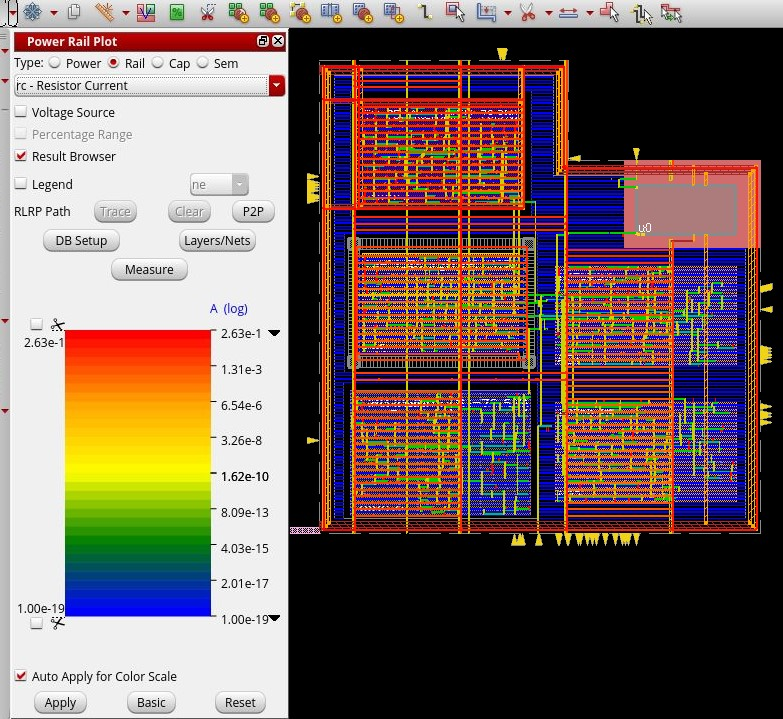
\includegraphics[width=.9\linewidth]{./img/era4.jpg}
\caption{\label{fig:orgb7b50f9}500mA on M5: Cell instances versus current consumption plot ( Resistor current)}
\end{figure}

\begin{figure}[htbp]
\centering
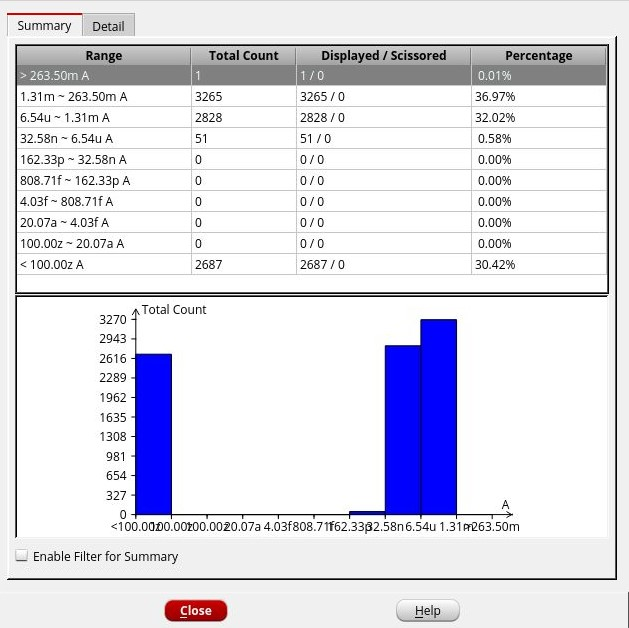
\includegraphics[width=.9\linewidth]{./img/era5.jpg}
\caption{\label{fig:orgd483690}500mA on M5: Cell instances versus current consumption plot ( Resistor current)}
\end{figure}


\begin{verse}
\vspace*{1em}
set\_rail\_analysis\_mode $\backslash$                                \#explaining analysis mode\\
\hspace*{3em}-method era\_static -accuracy xd $\backslash$                    \#analysis method static\\
\hspace*{3em}-extraction\_tech\_file ../data/qrc/gpdk090\_91.tch /   \#technology file 90nm\\
\hspace*{3em}-temperature 125 -analysis\_view AV\_wc\_on /\\
\hspace*{3em}-vsrc\_search\_distance 50\\
\hspace*{3em}-era\_current\_region\_file VSS.curRegion\\
set\_pg\_nets $\backslash$\\
\vspace*{1em}
\hspace*{4em}-net VSS -voltage 0 -threshold 0.05\\
\vspace*{1em}
\vspace*{1em}
set\_power\_data -reset\\
set\_power\_data -format ascii -scale 1 -bias\_voltage 0.05 VSS.curRegion\\
\vspace*{1em}
set\_power\_pads -reset\\
set\_power\_pads -format xy -file ../design/super\_filter\_VSS.pp -net VSS\\
\vspace*{1em}
analyze\_rail $\backslash$\\
\hspace*{3em}-type net -output ./era\_vss VSS\\
\vspace*{1em}
\end{verse}


\subsubsection{method}
\label{sec:org381e4d7}
\begin{figure}[htbp]
\centering
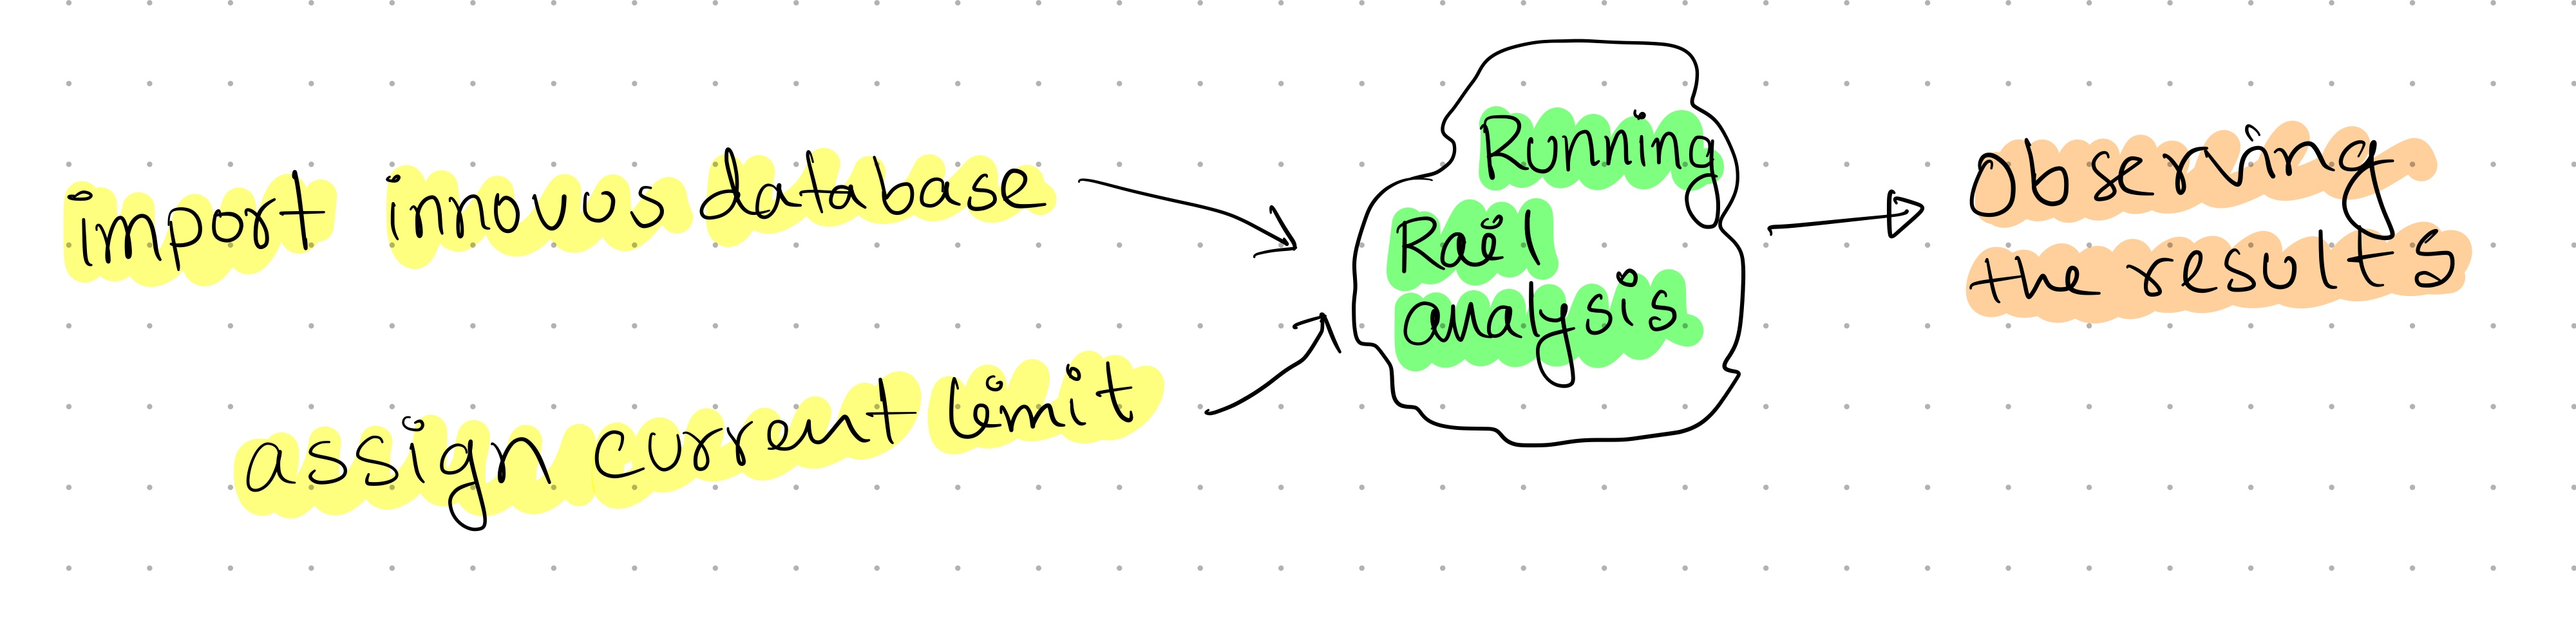
\includegraphics[width=.9\linewidth]{./img/era1.JPG}
\caption{\label{fig:org07ec07c}This is the caption for the next figure link (or table)}
\end{figure}


\subsection{Benchmark circuit}
\label{sec:orgc768bba}
I was trying to compare my design with benchmark circuit from Literature review. git-hub site file list.
\begin{itemize}
\item b19.bench
\item b19.blif
\item b19.edf
\item b19.fau
\item b19.vhd
\item b19\_C.bench
\item b19\_C.blif
\item b19\_C.edf
\item b19\_C.fau

\item b19 benchmark circuits(Viper and 80386 microprocessor)
\end{itemize}
\url{https://www.cerc.utexas.edu/itc99-benchmarks/polibench.pdf}

\section{Simulation: RISCV \& DNN Accelerator}
\label{sec:orgabfb093}

\subsection{DNN Accelerator GEMMINI IR DROP ANALYSIS.}
\label{sec:org0771867}
Steps
\begin{itemize}
\item Synthesize the RTL using PDK45
\item Used PDK45 lib and lef file for flooePlan
\item Extract tech library view and std library view files using QRC tech file (which I found in PDK45)
\item In floorPlan, I used extend to boundary for both vss and vdd stripe that will automatically implement VDD and VSS physical pad cell by default.
\item Early Rail Analysis (ERA) of GEMMINI \href{./innovus\_rail\_analysis.tcl}{tcl script}
\item Here is the report and IR drop distributions for VSS/ground bounce
\item \textbf{\textbf{1. Early Rail Analysis\_VSS\_rail}}
\end{itemize}
\begin{center}
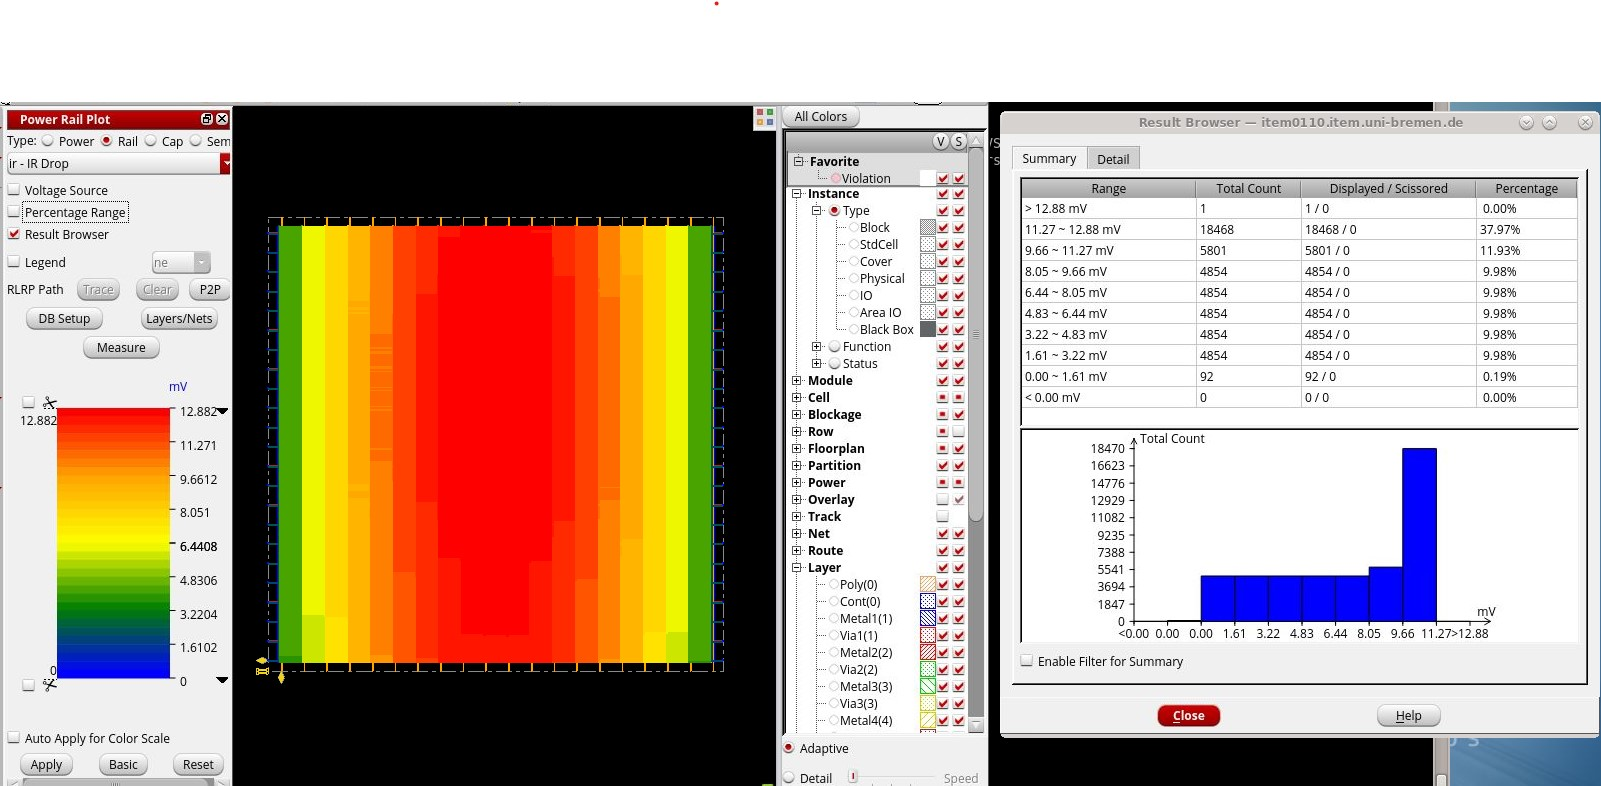
\includegraphics[width=.9\linewidth]{./img/ERA_VSS_Bounce_Gemmini.jpg}
\end{center}
\begin{itemize}
\item Report: IR drop for VSS \href{./rep/VSS.main.html}{Report}
\end{itemize}
\begin{center}
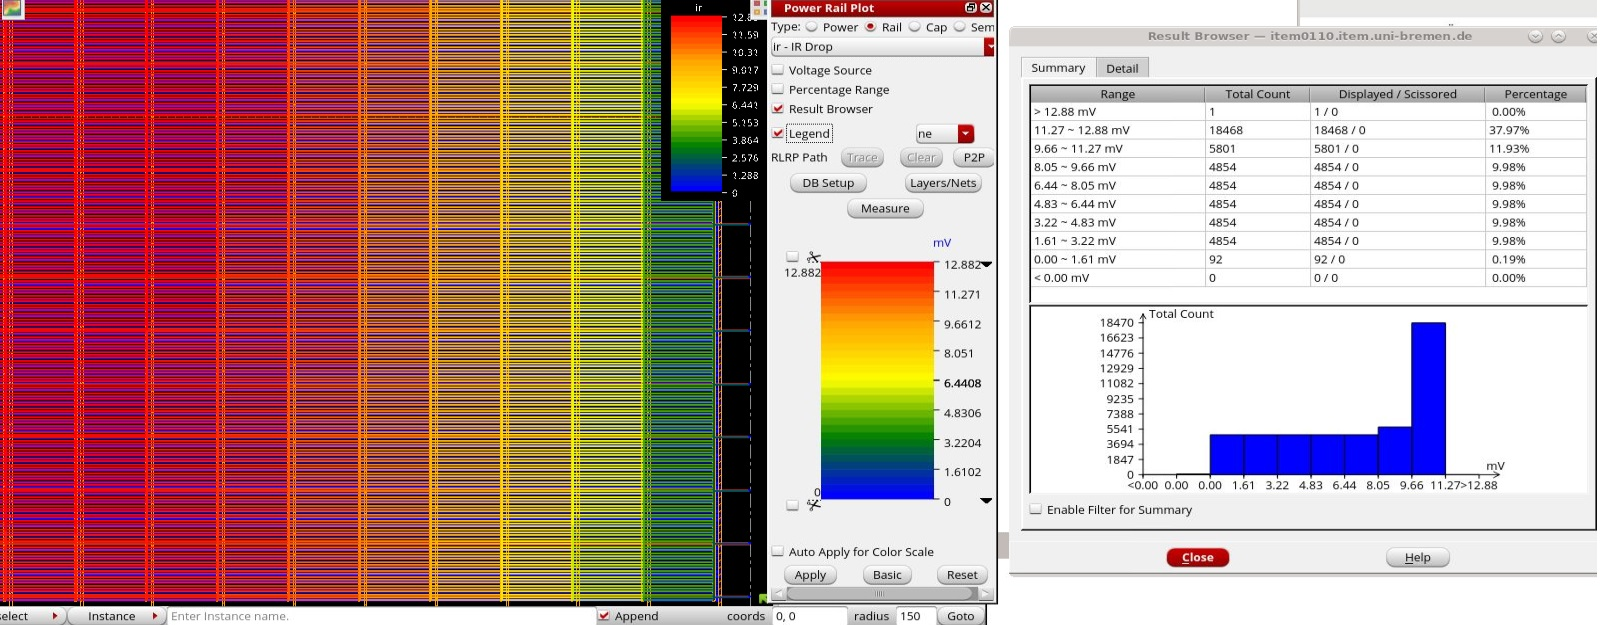
\includegraphics[width=.9\linewidth]{./img/vss_era.jpg}
\end{center}

\begin{itemize}
\item \textbf{\textbf{2. Early Rail Analysis\_VDD\_rail}}
\end{itemize}
\begin{center}
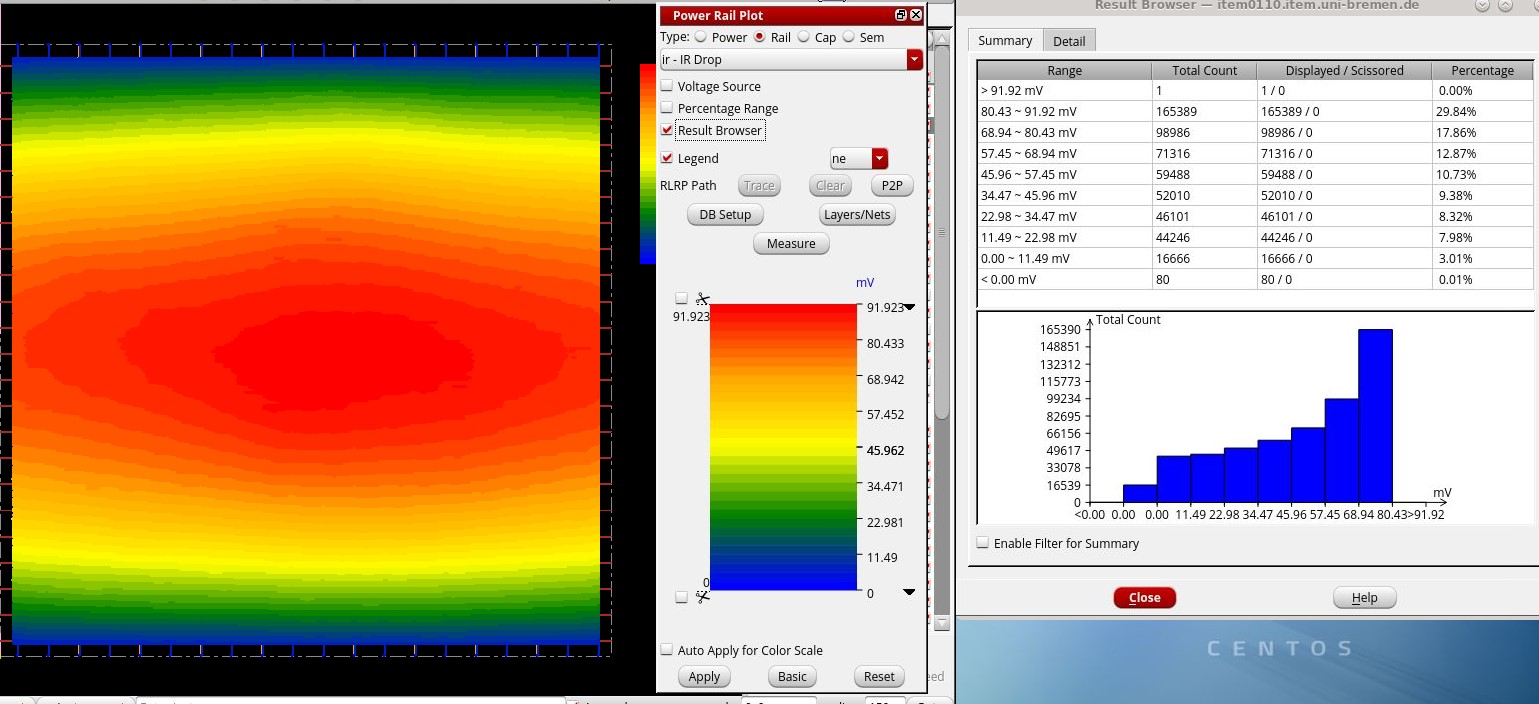
\includegraphics[width=.9\linewidth]{./img/gemmini_era2_vddd.jpg}
\end{center}
\begin{itemize}
\item Report: IR drop for VDD \href{./rep/VDD.main.html}{Report}
\end{itemize}
\begin{center}
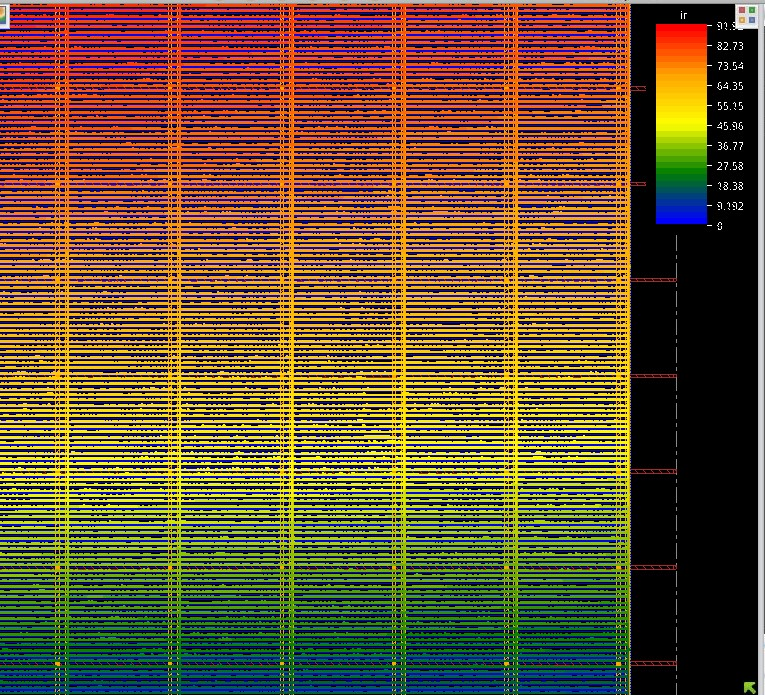
\includegraphics[width=.9\linewidth]{./img/gemmini_era2_vdd.jpg}
\end{center}






\noindent\rule{\textwidth}{0.5pt}
\subsubsection{Early Rail Analysis (ERA) of rocket core}
\label{sec:org55d519f}
\begin{itemize}
\item \textbf{\textbf{1. Early Rail Analysis\_VDD\_rail}}
\end{itemize}
\begin{center}
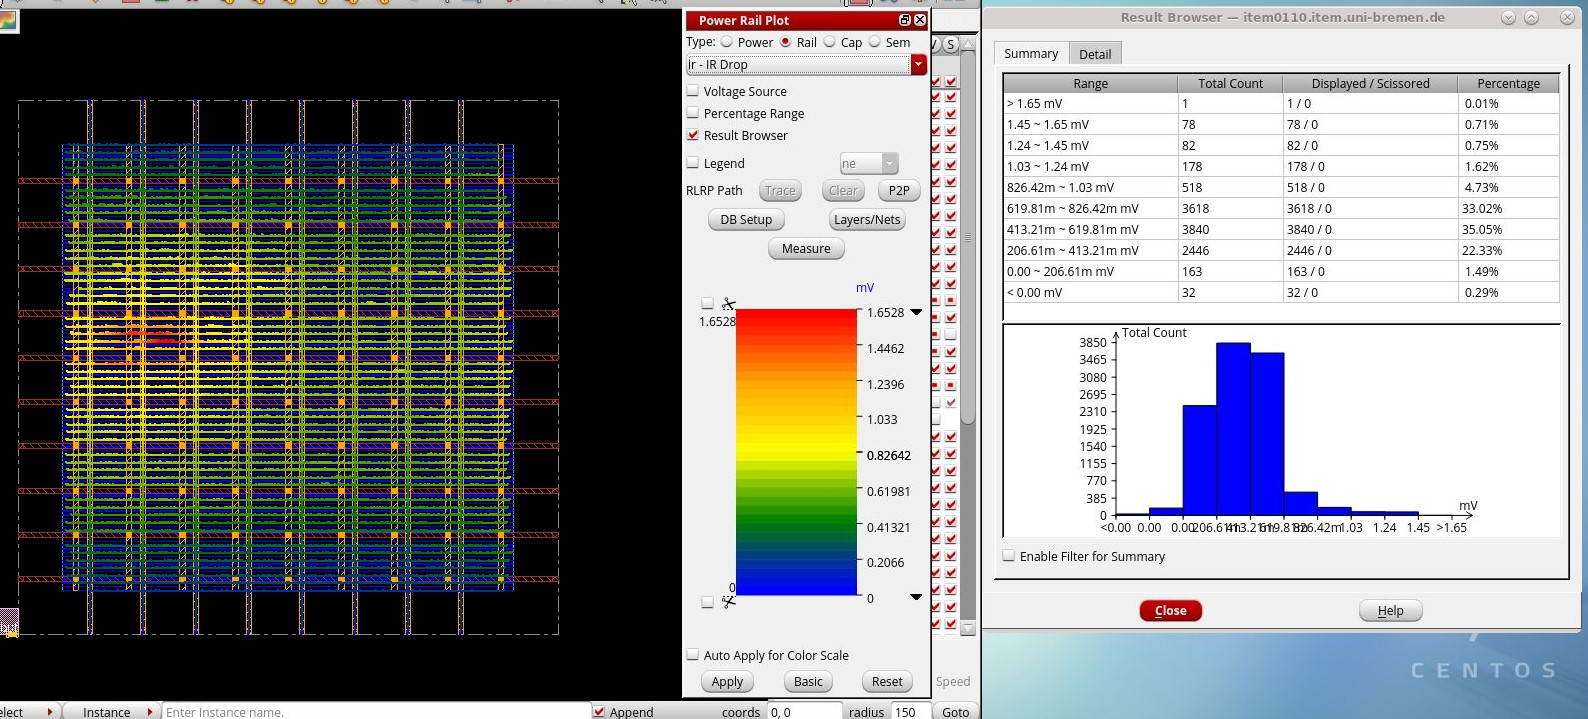
\includegraphics[width=.9\linewidth]{./img/rocket_era1_vdd.jpg}
\end{center}
\begin{itemize}
\item Report: IR drop for VDD \href{./rep/rocket\_VDD.main.html}{Report}
\end{itemize}
\begin{center}
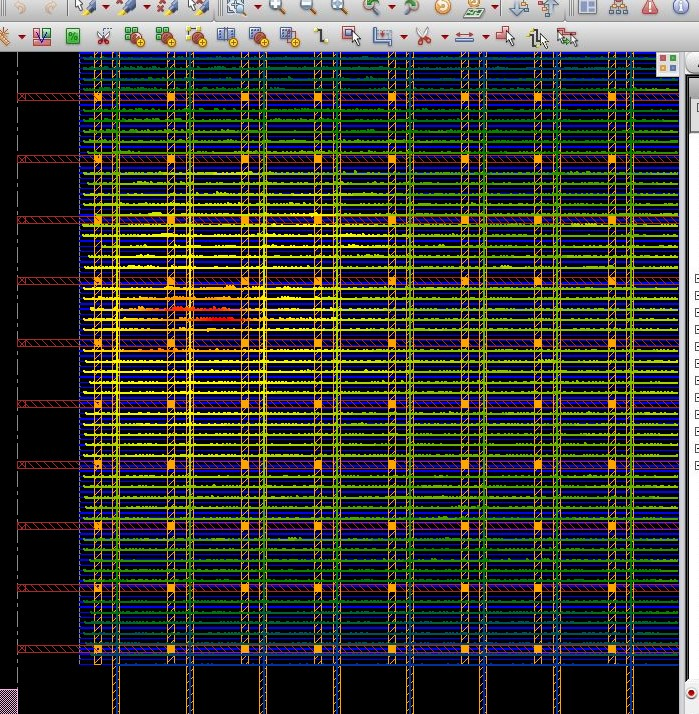
\includegraphics[width=.9\linewidth]{./img/rocket_era1_vddd.jpg}
\end{center}





\section{Personal Notes}
\label{sec:org6cbb1c5}

\subsection{Innovus Guide}
\label{sec:org1ff37fb}
\begin{itemize}
\item \href{./cpf\_sample.tcl}{CPF sample}
\item \href{./masterpnr.tcl}{PnR master script sample}

\item What is follow pin in VLSI physical design?
In VLSI physical design, a follow pin is a special type of pin used to
specify the routing direction of a net or signal. The follow pin is used
to guide the routing of a net, making sure that it follows a specific
direction or path.
\end{itemize}


Follow pins are often used in high-speed digital circuits, where the routing
of signals can significantly affect the performance of the circuit.
Designers may ensure that the signal takes the best path by setting
the routing direction of a net using a follow pin, lowering the chance of
crosstalk and other problems.

• innovus.cmd – Contains list of commands executed during the session. This file
can be used to create scripts to automate the execution of the commands and learn
what text commands correspond to commands executed through the GUI.
• innovus.log – Contains basic information output from the executed commands. The
commands in the file are preceded with in the file.
• innovus.logv – Similar to innovus.log but contains a more verbose amount of output. Useful for debugging


\subsection{Notes}
\label{sec:org4c54750}
\begin{itemize}
\item CPU Benchmarks
\begin{itemize}
\item Geekbench
\item Cinebench
\end{itemize}
\item GPU Benchmarks
\begin{itemize}
\item 3DMark
\item Unigine Heaven and Valley Benchmarks
\end{itemize}
\item Web Browser Benchmarks
\begin{itemize}
\item Octane and Kraken
\end{itemize}

\item There are two types of library file in VLSI
\begin{itemize}
\item Technology library (e.g
\item Cell library (eg nand, inverter)
\end{itemize}

\item EDIF file is a file format for transferring
design information between EDA vendors and EDA vendors and IC vendors
\item Berkeley Logic Interchange Format (BLIF)design information

\item Before starting the main design work check "Your INNOVUS have the required license for node tech,
\end{itemize}
maximum cell instance number and so on, Because innovus has a lot of different versions.

\begin{itemize}
\item definition file
\item design exchange file
\item chache parameter file
\item gz > GNU zip file
\item standard parasitic exchange format  spef file
\item power net power file  .ppfile
\item sdc >> synopsys design constraints file
\end{itemize}


\section{Question}
\label{sec:org1d49254}
\begin{itemize}
\item Which pdk I should use in b19?
\item not finding GPDK file TSMC 40nm and 65nm
\item need synthesis tool , design vision
\item Could you share me the lab file
\item UPF file is same as CPF file? both of the files are providing power details of chip.
\item definition.tcl or definition.view both are can be use as mmmc\_file for view analysis
\item Why we need to set init\_gnd and init\_pwr VDD and init\_gnd VSS in the time of design importing since we will provide cpf file (UPF file format can also be converted into cpf file, so chill both are kind of same) during imporing design.
\end{itemize}
cpf: It is an optional file for importing power domain configuration; Define different kind of power cell as like isolation cell and level shifter cell
and different rule, differnt power mode, always on cell, power clocking gate and so on.
and init power and gnd in the time of importing design is necessary this is how we initiate create power ring and stripes.


\subsection{Task}
\label{sec:org0936590}

\subsubsection{{\bfseries\sffamily TODO} [\#05] [DONE] Genus synthesis -> .v and .sdc file is ready}
\label{sec:orgfe6a51d}
\subsubsection{{\bfseries\sffamily TODO} [\#07] [DONE] Get for importing design}
\label{sec:org4979460}
\subsubsection{{\bfseries\sffamily TODO} [\#10] [DONE] Write floorplan script  in .tcl}
\label{sec:org1459713}
\subsubsection{{\bfseries\sffamily TODO} [\#20] [DONE] Write placement script in -tcl}
\label{sec:org223ac47}
\subsubsection{{\bfseries\sffamily TODO} [\#30] [DONE] Get ready for CTS script}
\label{sec:org2025cbf}
\subsubsection{{\bfseries\sffamily TODO} [\#40] [DONE] script for Routing}
\label{sec:orge411eff}
\subsubsection{{\bfseries\sffamily TODO} [\#55] [DONE] script for Optimization}
\label{sec:org24e5a51}
\subsubsection{{\bfseries\sffamily TODO} [\#65] [DONE] Def exporting script}
\label{sec:orgf2773a8}
\subsubsection{{\bfseries\sffamily TODO} [\#80] [DONE] save design in .enc format}
\label{sec:org58f589a}
Abdul Aziz_Project SoSe23
\end{document}
